Lui inizia alle 11.30 e finisce mezz'ora prima (13.00).

\section{Segnali tempo continuo e discreto}
Nella figura delle serie storiche e del suono del diapason la variabile indipendente (x) e' il tempo. Storicamente i segnali temporali sono quelli piu' vicini alla percezione della realta'.
Il segnale che abbiamo visto adesso aveva un andamento oscillatorio, ed abbiamo detto che e' a tempo continuo e quindi lo rappresentiamo come una funzione matematica x(t), quindi una funzione e' un segnale, noi parleremo di funzioni che descrivono situazioni reali con caratteristiche particolari.
Il tempo per un segnale a tempo continuo perche' appartiene all'insieme dei numeri reali (R), $t \in \mathbb R$.
In realta' i segnali sono creati da dei campioni distanziati da un certo intervallo (segnali a tempo discreto) che chiameremo genericamente $\Delta (t)$, andiamo a far crescere il numero del campione man mano che progrediamo, quindi la variabile a indipendente e' n, e la funzione dipende da n: x[n], parleremo di funzione discreta usando le parentesi quadre. (e' un segnale a tempo discreto con variabile indipendente n).

\begin{figure}[ht!]
    \centering
    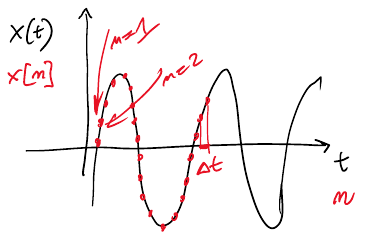
\includegraphics{immagini/lez1/segnaleTempoContinuo.jpg}
    \caption{Segnale a tempo continuo vs tempo discreto}
    \label{fig:tempoContinuo}
\end{figure}

Noi ci occuperemo di segnali monodirezionali, la variabile indipendente sara' 1, nel caso appena visto il tempo. Esistono anche segnali in cui ci sono piu' variabili indipendenti, l'immagine.

\begin{figure}[ht!]
    \centering
    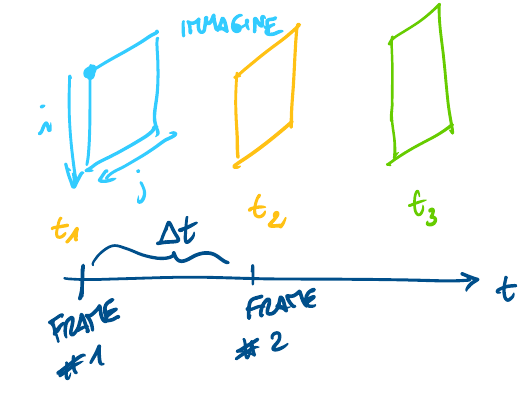
\includegraphics[scale=0.75]{immagini/lez1/segnaliMultidirezionali.jpg}
    \caption{Segnali multidirezionali}
    \label{fig:multidirezionali}
\end{figure}

Abbiamo un indice j che indica la riga ed un sensore i che indica la colonna, abbiamo due variabili indipendenti di tipo spaziale e se introduciamo un'altra variabile indipendente il tempo otteniamo una sequenza di immagini che e' un video: nel video abbiamo una variabile a tempo continuo che cresce (il tempo) che viene discretizzato in tutti i frame, e tra tutti i frame ci sara' un $\Delta t$. In questo caso abbiamo un segnale tridimensionale con 2 variabili indipendenti spaziali ed 1 variabile indipendente temporale.

\section{Sistema}
Cio' che manipola un segnale tipicamente si chiama sistema, che cos'e' un sistema?
Per adesso lo rappresentiamo come una scatola che e' il nostro algoritmo che ha in ingresso il nostro segnale tempo discreto x[n] ed in uscita ha un altro segnale tempo discreto y[n], cosa succede all'interno dell'algoritmo al momento non ci interessa, ma sappiamo che il segnale viene modificato, consideriamo che l'algoritmo sia una funzione y[n] = T{x[n]}.

\begin{figure}[ht!]
    \centering
    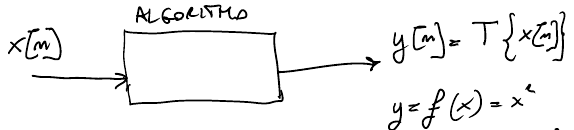
\includegraphics[scale=0.75]{immagini/lez1/sistema.jpg}
    \caption{Sistema}
    \label{fig:sistema}
\end{figure}

\section{Segnali e Sistemi}
Abbiamo i segnali che all'inizio saranno a tempo continuo, impareremo le caratteristiche di questi segnali ed impareremo a convertirli in tempo discreto con un convertitore analogico digitale, all'uscita di questo convertitore avremo un segnale a tempo discreto. Questo segnale tempo discreto impareremo a manipolarlo con un sistema che ci da un segnale in uscita che ancora una volta e' a tempo discreto. 
Per ora siamo ancora in un mondo a tempo discreto, pero' la nostra applicazione deve fare qualcosa nel mondo reale, allora in questo caso dobbiamo tornare nel tempo continuo, lo facciamo con un convertitore digitale analogico(DAC), quindi in uscita avremo un segnale a tempo continuo.

\begin{figure}[ht!]
    \centering
    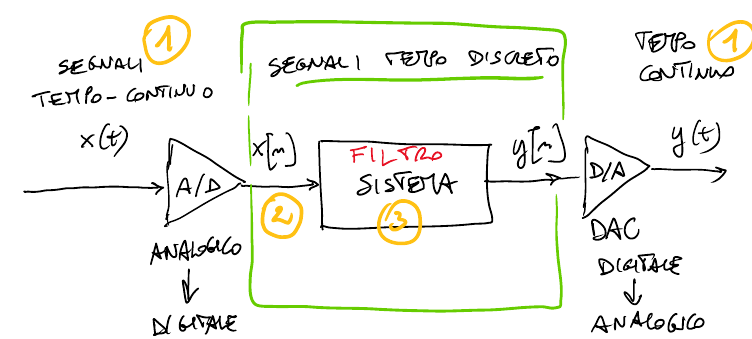
\includegraphics[scale=0.75]{immagini/lez1/continuoAdiscreto.jpg}
    \caption{Trasformare i segnali da tempo continuo a discreto}
    \label{fig:continuoAdiscreto}
\end{figure}

Dobbiamo partire dai segnali tempo continui perche' vogliamo capire che segnali digitali li caratterizzano, dopo di che parleremo dei segnali digitali, a questo punto potremo manipolare i segnali digitali parlando dei sistemi.
Infine torneremo ai segnali perche' vorremo essere in grado non solo di capire come funziona un sistema ma anche di progettarlo.
Un'altro modo di dire la parola sistema e' FILTRO, quindi dovremo essere in grado di scrivere degli algoritmi che siano dei filtri digitali che trasformino il segnale come vogliamo noi, lo faremo soprattutto nel contesto di Fourier.

\section{Segnale trigonometrico}
Nel contesto dei segnali tempo continui andiamo a ripassare un segnale trigonometrico, il piu' semplice e' il coseno:
\begin{equation}
    x(t) = A_0 \cos(2\pi f_0 t + \varphi_0)
\end{equation}

ricordiamo che t e' la variabile indipendente e non e' un parametro, certamente al variare di t cambia il segnale, ma siamo interessati al segnale nella sua interezza.

Andiamo ora a definire meglio tutti i parametri dell'equazione appena vista.

\subsection{Ampiezza}
 $A_0$ e' l'ampiezza del segnale, moltiplicare il coseno per un ampiezza significa aumentare o diminuire i punti massimi del coseno. Se $A_0 > 1 $ aumento i punti massini, altrimenti li diminuisco.

\subsection{Frequenza}
$f_0$ e' la frequenza del segnale cosinusoidale (in questo caso solo 1). Il concetto di frequenza e' un concetto base (con che frequenza mangi in una giornata), intendiamo il numero di volte che facciamo qualcosa in un unita' di tempo, per quanto ci riguarda la nostra unita' di tempo e' 1 secondo. Si misura in Heartz (hz) ed e' ottenuta dal numero di eventi fratto l'unita' di tempo. Nel nostro caso dato che stiamo parlando di un coseno, il quale e' periodico di periodo $2 k \pi$, questo sara' uguale a se stesso (si ripetera')dopo:

\begin{equation}
    2\pi f_0 t + \varphi_0 = 0 + 2 \pi k + \varphi
\end{equation}

dove k e' una costante e $k \in \mathbb(Z)$.
Da questa formula posso quindi scrivere che $t =\frac{k}{f_0} = k T_0$.
Dove $T_0 = \frac{1}{f_0}$ che e' il periodo del segnale.
Il segnale si ripetera' un'infinita' di volte, ma e' un modello.
Questo $f_0$ diremo indicativamente che e' grande per segnali ad alta frequenza, in questo caso se la frequenza e' grande il periodo (inverso della frequenza) sara' piccolo. Avremo anche segnali a bassa frequenza con $f_0$ piccolo ed il periodo grande. Queste stesse cose valgono anche per la lunghezza d'onda nelle radio.

\subsection{Pulsazione}
Un altra grandezza da considerare e' la pulsazione (frequenza angolare o velocita' angolare), generalmente detta $\omega_0$ ed e' banalmente uguale a $2\pi \cdot f_0$, cioe' portiamo in radianti la frequenza.
Si misura di conseguenza in radianti al secondo: $\frac{\mbox{RAD}}{1}$.
Soprattutto nel tempo discreto la velocita' angolare si usa molto, perche' viene riportata al concetto di frequenza.

\subsection{Fase}
$\varphi_0$ e' la fase, sposta il segnale a destra o sinistra rispettivamente se positiva o negativa. Ricordiamoci sempre che stiamo lavorando con segnali periodici, quindi potremo spostarli fino a $2\pi$, dopo di che tornano ad essere uguali, quindi generalizzando il concetto possiamo dire che tutto quello che esce dal range $0 \rightarrow 2\pi$ non modifica la funzione, una conseguenza di questa cosa e' che data una funzione periodica possiamo rimapparla togliendo $2\pi$.
In elaborazione dei segnali, per convenzione, si preferisce considerare il periodo base $-2\pi \rightarrow \pi$.

Nell'esempio vediamo come sommare o sottrarre una costante $\tau = 2$ trasla rispettivamente a destra e sinistra la funzione, esattamente il comportamento che ha la fase.

\begin{figure}[ht!]
    \centering
    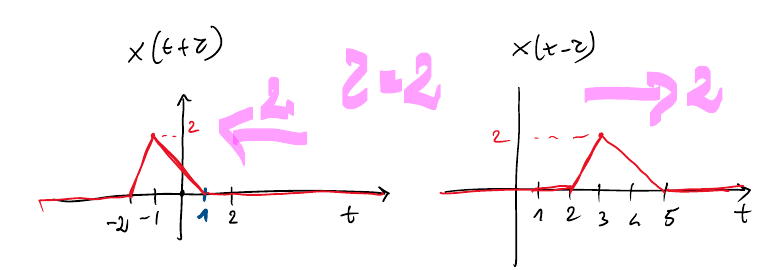
\includegraphics[scale=0.75]{immagini/lez1/modificareTempo.jpg}
\end{figure}

